%\section{Understanding and Modeling Transient Server Preemptions}
%\section{Modeling the Dynamics of Transient Server Preemptions}
%\section{Preemption Dynamics of Transient Cloud Servers}
%\vspace*{\subsecspace}
% \section{Constrained Preemptions of Google Preemptible VMs} %sigmetrics
\section{Understanding temporally constrained VM preemptions}
\label{sec:failmodel}

%Understanding the nature and dynamics of transient cloud servers such as their preemption frequency is a prerequisite to understand and improve the performance of applications.

%This is presumably in the background 
\eat{In order to understand and improve the performance of applications running on transient cloud servers, we must understand the nature and dynamics of their preemptions.
The preemption characteristics are governed by the supply of surplus resources, the demand for cloud resources, and the resource allocation policies enforced by the cloud operator.
Therefore, in this section, we present empirical and analytical models to help us understand the nature of preemptions. 
}

%To measure and improve the performance of applications running on transient cloud VMs, it is critical to understand the nature and dynamics of their preemptions.
%

In our quest to understand temporally constrained preemptions, we  conduct an empirical study of preemptions of Google Preemptible VMs.
Based on our observations and insights from the study, we then develop a probability model for temporally constrained preemptions, which we later use to develop preemption-mitigating resource management application policies. 




%In this section, we first present an empirical analysis of preemptions of Google Preemptible VMs, and then develop a new  probability model based on our observations. 
%Finally, we discuss the unique aspects and general characteristics of constrained preemptions using reliability theory. % and statistical mechanics.


%and present  general observations about constrained preemptions using statistical mechanics. 

%The preemption characteristics are governed by the supply of surplus resources, the demand from applications, and resource allocation policies of the cloud operator.


%that describe these characteristics and enable an intuitive understanding of the nature of preemptions. 


% Transient cloud servers, by their very nature have limited availability and are frequently preempted.
% These preemptions are akin to fail-stop failures, and are often preceeded by a small advance warning (few seconds) to allow for graceful shutdowns.

% Since preemptions can impact the availability, performance, and cost of running applications, in this section, we examine their preemption characteristics.
% This modeling is important, because having a model of the availability can be useful in the context of predicting the running times of applications.
% Cloud providers offer a large number of servers of different configurations and types.
% Since transient server availability is fundamentally tied to supply and demand, the availability of servers of different types can be significantly different. 
% Thus, selecting the ``right'' server type is crucial for minimizing the overall costs. 



%\cite{alicloud-spot, packet-spot}

%\subsection{Empirical model of preemptions}
%\subsection{Empirical preemption behavior}
\vspace*{\subsecspace}
\subsection{Empirical Study Of Preemptions}\label{sec:empirical}
%\subsection{Understanding Empirical Preemption Behavior}

% The preemptions of transient servers need not be related to their price.

\begin{figure}
  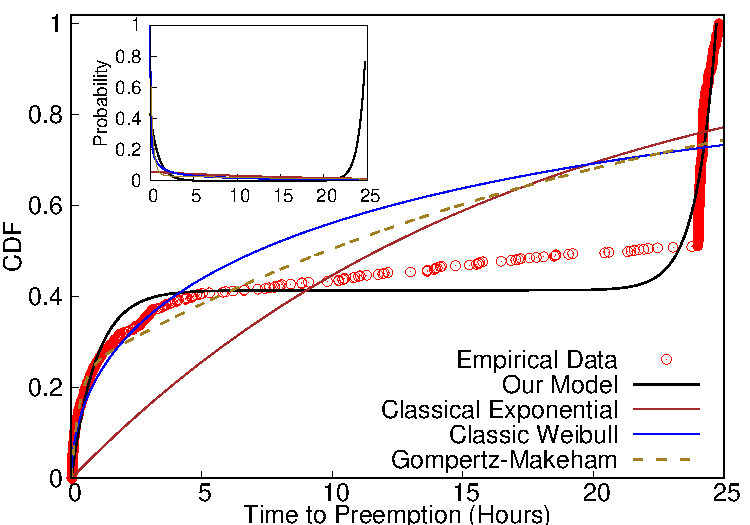
\includegraphics[width=0.47\textwidth]{../data/gnuplot-figures/sigmetrics-fig-cdf-prob-inset-time.pdf} 
  \caption{CDF of lifetimes of Google Preemptible VMs. Our proposed distribution for modeling the constrained preemption dynamics provides a better fit to the empirical data compared to other failure distributions. Inset shows the probability density functions.}
  \label{fig:gcp1}
\end{figure}

%To understand the nature of temporally constrained preemptions, we conducted an empirical study of Google's Preemptible VMs, that have a fixed price and a maximum 24 hour lifetime. 
%Our empirical approach is necessary since the cloud operator (Google) does not disclose any other information about the preemption rates, and thus relatively little is known about the preemptions of these VMs. 


\noindent \textbf{Methodology.}
We launched  870 Google Preemptible VMs of different types over a two month period (Feb--April 2019), and measured their time to preemption (i.e., their useful lifetime).
%
VMs of different resource capacities were launched in a four geographical regions; during days and nights and all days of the week; and running different workloads\footnotemark. 
%hl
We launched VMs in their default resource configurations (CPU and memory), and do not use custom VM sizes.
% hl
% Explain which ones? regions and instance types? 
%\vikram{We analyzed a subset (870) of this data to see how launched VMs are distributed across seven days of the week. We found the following distribution: Monday: 81, Tuesday: 204, Wednesday: 181, Thursday: 82, Friday: 144, Saturday: 124, and Sunday: 54.
%We also analyzed the distribution of this data across 4 hour period in a day: 0-4: 20, 4-8: 75, 8-12: 331, 12-16: 223, 16-20: 117, and 20-24: 104.
%We experimented with different CPU types with differnt size of memory such as n1-highcpu-2: 1.80GB, n1-highcpu-4: 3.60GB, n1-highcpu-8: 7.20GB, n1-highcpu-16: 14.4GB, n1-highcpu-32: 28.8GB, and n1-highcpu-64: 57.6GB.}
To ensure the generality of our empirical observations, VMs were not launched during well-known peak utilization days (such as Black Friday).
%
The preemption data collection was bootstrapped: a small amount of data points were used to estimate and model the preemption CDF, which we then used to run our batch computing service (described and evaluated in Sections~\ref{sec:impl} and \ref{sec:eval}), which generated the rest of the preemption data.  
%
%Thus the effective cost overhead of our empirical data collection approach  is small. 
Due to the relatively high preemption rates compared to EC2 spot instances, we were able to collect these data points for less than \$5,000. 
%

\footnotetext{Preemption rates can also be affected by number of VMs launched simultaneously, which we limited to between $1$ and $10$.}

%
 %Weaksauce 
%
A sample of over 100 such preemption events are shown in Figure~\ref{fig:gcp1}, which shows cumulative distribution function (CDF) of the lifetime of the \texttt{n1-highcpu-16} VM in the \texttt{us-east1-b} zone. 
%enter the type of VM for which the data is shown
%
Our empirical approach allows us to make the following  observations.

%Based on the observ
%
%Note that the cloud operator (Google) caps the \emph{maximum} lifetime of the VM to 24 hours, and all the VMs are preempted before that limit. 

\begin{figure*}
  %\centering
  \subfloat[Preemption characteristics of different VM types. Larger VMs are more likely to be preempted.
  \label{fig:cdf-comparison}]
  {  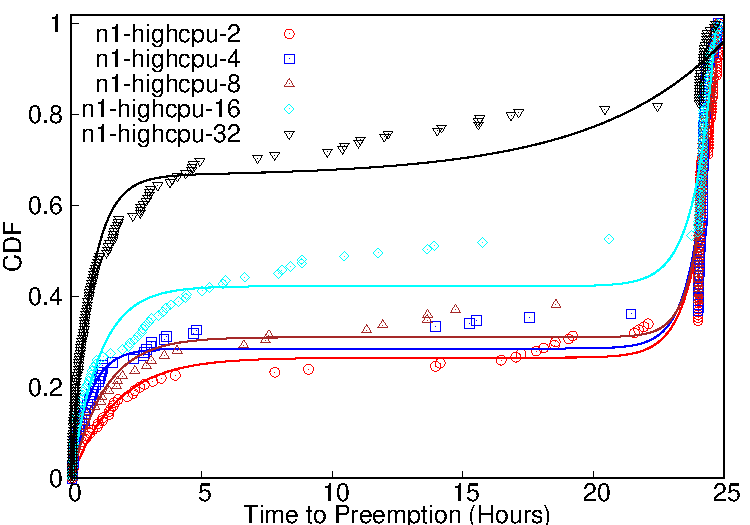
\includegraphics[width=0.3\textwidth]{../data/gnuplot-figures/sigmetrics-fig-vm-types.pdf} }
  \hfill
\subfloat[Variations due to time of day and workload. \label{fig:time-breakdown}]
{  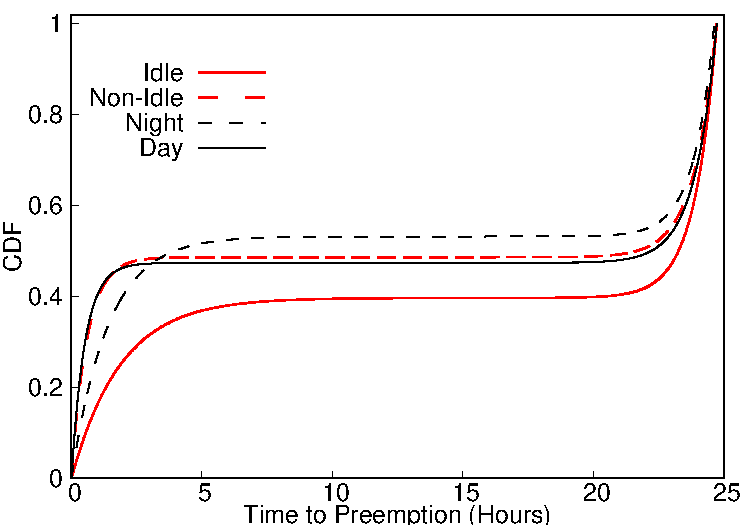
\includegraphics[width=0.3\textwidth]{../data/gnuplot-figures/sigmetrics-time-breakdown.pdf} }
\hfill
\subfloat[\textbf{n1-highcpu-16} in different regions. \label{fig:region-breakdown}]
{  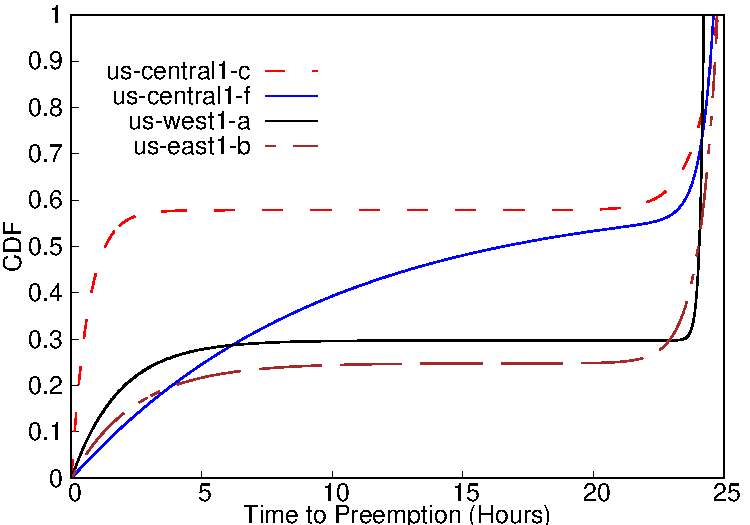
\includegraphics[width=0.3\textwidth]{../data/gnuplot-figures/sigmetrics-region-breakdown.pdf} }
\vspace*{-0.6cm}
\caption{Analysis of preemption characteristics by VM-type, region, time-of-day, and workload type.}
\label{fig:breakdown-all}
    \vspace*{\myfigspace}
\end{figure*}

\noindent \textbf{Observation 1:} \emph{The lifetimes of VMs are not uniformly distributed, but have three distinct phases.}

\noindent In the first (initial) phase, characterized by VM lifetime $t\in [0, 3]$ hours, we observe that many VMs are quickly preempted after they are launched, and thus have a steep rate of failure. The rate of failure (preemption rate) is the derivative of the CDF.
%; the rate of failure or preemptions can be obtained by taking the derivative of the CDF. 
The early high rate of failure reflects that the cloud service provider takes into account VM liftetime in prioritizing preempting ``younger'' VMs, in other words, the number of simultaneous VMs launched does have an effect on their failure rate. 
%
In the second phase, VMs that survive past 3 hours enjoy a relatively low preemption rate over a relatively broad range of lifetime (characterized by the slowly rising CDF in Figure~\ref{fig:gcp1}).
The third and final phase exhibits a steep increase in the number of preemptions as the preemption deadline of 24 hours approaches.
The overall rate of preemptions is ``bathtub'' shaped as shown by the solid black line in the inset of Figure~\ref{fig:gcp1} (discussed in detail below).
%\it I think we should show the probability plot to exhibit the bath tub shape

%The preemption rate is ``bath tub'' shaped, with VMs that survive past 3 hours enjoying a relatively low preemption rate, and finally a steep increase in the number of preemptions as the preemption deadline (24 hours) approaches. 


\noindent \textbf{Observation 2:} \emph{The preemption behavior, imposed by the constraint of the 24 hour lifetime, is substantially different from conventional failure characteristics of hardware components and EC2 spot instances.}

\noindent In ``classical'' reliability analysis, the rate of failure  usually follows an exponential distribution $f(t) = \lambda e^{-\lambda t}$, where $\lambda=1/\text{MTTF}$.
Figure~\ref{fig:gcp1} shows the CDF ($=1-e^{-\lambda t}$) of the exponential distribution when fitted to the observed preemption data, by finding the distribution parameter $\lambda$ that minimizes the least squares error.
The classic exponential distribution is unable to model the observed preemption behavior because it assumes that the rate of preemptions is independent of the lifetime of the VMs, i.e., the preemptions are \emph{memoryless}.
%The primary reason is that the exponential distribution assumes that the \vj{the rate of preemptions is independent of the lifetime of the VMs} (preemptions are \emph{memoryless}), which does not hold true when there is a fixed upper bound on the lifetime, as is the case for Google Preemptible VMs. \vj{In other words, the conventional approach is insufficient to model constrained preemption dynamics.}
%We attribute this deficiency to the central assumption made in the underlying reliability theory principles that leads to the classical exponential distribution: the rate of preemptions is independent of the lifetime of the VMs, in other words, the preemptions are \emph{memoryless}.
This assumption breaks down when there is a fixed upper bound on the lifetime. %, as is the case for Google Preemptible VMs.%, and the conventional approach becomes insufficient to model this constrained preemption dynamics. 

\noindent \textbf{Observation 3:} \emph{The three preemption phases and associated bathtub shaped preemption probability are general, universal characteristics of Preemptible VMs.}

%In general, the preemption dynamics of a VM are determined by the supply and demand of VMs of that \emph{particular} type. 
%Thus, o
Our empirical study looked at preemptions of VMs of different sizes (Figure~\ref{fig:breakdown-all}a), at different times of the day (Figure~\ref{fig:breakdown-all}b), in different geographical zones (Figure~\ref{fig:breakdown-all}c), and running different workloads. 
In all cases, we find that there are three distinct phases associated with the preemption dynamics giving rise to the bathtub shaped preemption probability. 


\noindent \textbf{Observation 4:}\emph{ Larger VMs have a higher rate of preemptions.}

Figure~\ref{fig:cdf-comparison} shows the preemption data from five different types of VMs in the Google Cloud \texttt{n1-highcpu-\{2,4,8,16,32\}}, where the number indicates the number of CPUs.
All VMs are running in the \texttt{us-central1-c} zone. 
We see that the larger VMs (16 and 32 CPUs) have a higher probability of preemptions compared to the smaller VMs.
While this could be simply due to higher demand for larger VMs, it can also be explained from a cluster management perspective. 
Larger VMs require more computational resources (such as CPU and memory), and when the supply of resources is low, the cloud operator can quickly reclaim a large amount of resources by preempting larger VMs.
This observed behavior aligns with the guidelines for using preemptible VMs that suggests the use of smaller VMs when possible~\cite{preemptible-documentation}. 

\noindent \textbf{Observation 5:} \emph{Preemptions exhibit diurnal variations, and are also affected by the workload inside the VM.}

From Figure~\ref{fig:time-breakdown}, we can see that VMs have a slightly longer lifetime during the night (8 PM to 8 AM) than during the day\footnotemark. 
This is expected because fundamentally, the preemption rates are higher during periods of higer demand. 
%
We also notice that completely idle VMs have longer lifetimes than VMs running some workload.
Presumably, this could be a result of the lower resource utilization of idle VMs being more amenable to resource overcommitment, and result in lower preemptions. 


\footnotetext{Time-zone local to the VM's location.}

% \begin{figure}
%   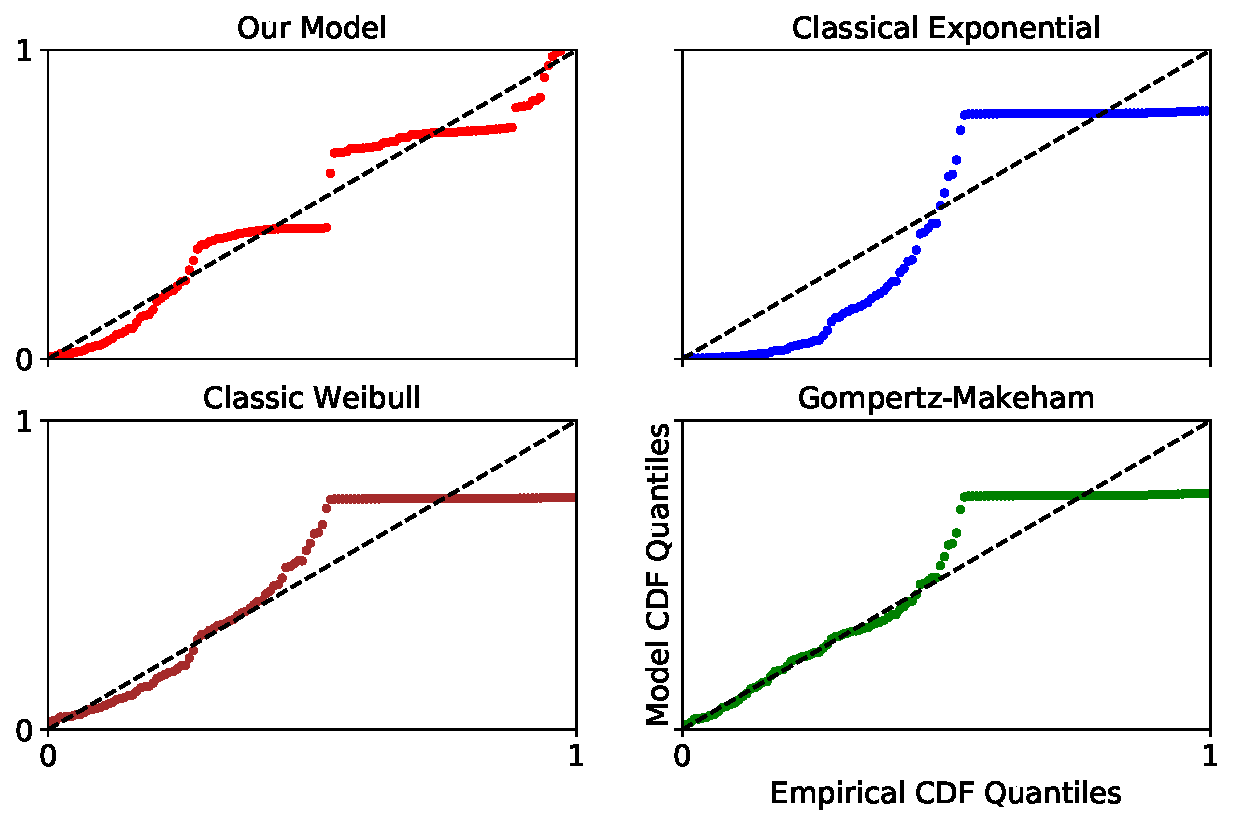
\includegraphics[width=0.4\textwidth]{../graphs/QQ.pdf}
%     \vspace*{-5pt}
%     \caption{QQ plot of different preemption models. Weibull and Gompertz-Makeham can model preemptions up to CDF=0.5, but not over the entire range.}
%       \vspace*{-7pt}
%       %Existing models are unable to capture all the preemption phases.}
%   \label{fig:QQ}
%   \vspace*{-5pt}
% \end{figure}

%being more amenable to resource overcommitment, and therefore don


%\noindent \textbf{Why temporal constraints result in bathtub preemptions.}

\noindent \textbf{Significance of bathtub preemptions.} 
The above empirical observations indicate that temporally constrained preemptions are \emph{not} uniformly distributed. 
%
The bathtub shaped preemption distribution is not a coincidence.
It is a result of fundamental characteristics of constrained preemptions that benefit applications. 
%We argue that this is not a coincidence, but may be a result of practical and fundamental outcomes of cluster management policies. 
%
%While the actual specific preemption policy is up to the cloud operator, we will show that the bathtub behavior has benefits for applications. 
%The bathtub behavior results in a high rate of failure initially. 
For applications that do not incorporate explicit fault-tolerance (such as checkpointing), early preemptions result in less wasted work than if the preemptions were uniformly distributed over the 24 hour interval.
%
Furthermore, the low rate of preemptions in the middle periods allows jobs that are smaller than 24 hours to finish execution with only a low probability of failure, once they survive the initial preemption phase. 
%
We compare application performance with bathtub preemptions and uniformly distributed preemptions later in Section~\ref{sec:eval}, and find that bathtub preemptions can reduce the performance overheads of preemptions by up $10\times$.
%
However, effective policies for constrained preemptions  requires a probability model of preemptions, which is challenging due to the temporal constraint and the steep bathtub behavior. 
%
Existing preemption models are not applicable, and we present our new model next. 


%But can improve runtime by as much as 4x compared to uniform preemption rates. 
%
%In addition to being beneficial to applications, we also conjecture that the bathtub behavior may be  a \emph{fundamental} and general characteristic of constrained preemptions, which we show later in Section~\ref{subsec:stat-mech}. 
%system where events are randomly distributed in a finite interval later in Section~\ref{subsec:stat-mech}. 
%
%Intriguingly, we can analyze such temporally constrained preemptions through a statistical mechanics framework, and we elaborate on this connection later in Section~\ref{subsec:statmech}.




%%%%%%%%%%%%%%%%%%%%%%%%%%%%%%%%%%%%%%%%%%%%%%%%%%%%%%%%%%%%%%%%%%%%%%

\vspace*{\subsecspace}
\subsection{Failure Probability Model}
\label{subsec:analytical-model}

%Based on our empirical analysis of preemptions,  
We now develop an analytical probability model for finding a preemption at time $t$ (preemption dynamics) that is faithful to the empirically observed data and provides a basis for developing running-time and cost-minimizing optimizations. %
%
% Something about generalizability etc.
% 
Modeling preemptions constrained by a finite deadline raises many challenges for existing preemption models that have been used for other transient servers such as EC2 spot instances.
%
We first discuss why existing approaches to preemption modeling are not adequate, and then present our closed-form probability model and associated reliability theory connections. 

%How to avoid sounding like the background section?

% Motivations and requirements from a new model? Capture all these observations : differences, and also the general bathtub distribution. 
\vspace*{\subsecspace}
\subsubsection{Inadequacy of existing failure distributions}

Spot instance preemptions have been modeled using exponential distribution~\cite{bid-cloud, hotcloud-not-bid, flint}, which is the default in most reliability theory applications. 
However, the strict 24 hour constraint and the distinct preemption phases are not compatible with the memoryless properties of the exponential distribution. 
%
To describe failures (preemptions) that are not memoryless (i.e., increasing or decreasing failure rate over time), the classic Weibull distribution with CDF $F(t)=1-e^{-(\lambda t)^k}$ is often employed. However, the Weibull distribution is also unable to fit the empirical data (Figure~\ref{fig:gcp1}) and especially unable to model the sharp increase in preemptions near the 24 hour deadline. 

For constrained preemptions, the increase in failure rate as modeled by the Weibull distribution is not high enough.
Other distributions, such as Gompertz-Makeham, have also been used for modeling bathtub behavior, especially  for actuarial use-cases~\cite{missov2013gompertz}. 
The key idea is to incorporate an exponential aging process, which is used to model human mortality.
The CDF of the Gompertz-Makeham distribution is given by $F(t) = 1 - \exp\left(-\lambda t - \dfrac{\alpha}{\beta}(e^{\beta t} - 1) \right)$
and is fitted to the data in Figure~\ref{fig:gcp1}, and is also unable to provide a good model for the observed preemption data.
%


%Specifically, it is unable to model the bathtub preemption rate and the different preemption phases, and 


%We also analyze other distributions used for modeling bathtub failures from reliability and actuarial theory in Figure \textbf{XXX}.


The non-trivial bathtub-shaped failure rate (Figure~\ref{fig:gcp1}) requires models that capture the sudden onset of the rise in preemptions near the deadline, which is challenging for the existing failure distributions because of the sharp inflection point. 
From an application and transiency policy perspective, the preemption model must provide insights about the phase transitions, so that the application can adapt to the sharp differences in preemption rates.
%
For example, the preemption model should be able to warn applications about impending deadline, which existing failure distributions cannot account for. 
% which imposes a dynamics that is more akin to a constrained dynamics problem as opposed to dynamics characterized with a gradually rising failure rate.
Thus, not only is it important to minimize the total distribution fitting error, it is also important to capture the changes in phase.
%
However,
%as we can see from the QQ plots in Figure~\ref{fig:QQ},
existing distributions are unable to capture the effects of the deadline and all the phases of the preemptions, and a new modeling approach is needed. 

\vspace*{\subsecspace}
\subsubsection{Our  model}
\label{subsec:preemption-model}


%This is especially important from a policy design perspective, as the ``phase changes'' in preemption behavior can greatly affect the failure probability and performance of applications.
%Our new model, informed by the cumulative distribution of lifetimes that has multiple distinct temporal phases, addresses this need.

Our failure probability model seeks to address the drawbacks of existing reliability theory models for modeling constrained preemptions. 
The presence of three distinct phases exhibiting non-differentiable transition points (sudden changes in CDF near the deadline, for example) suggests that for accurate results, models that treat the probability as a step function (CDF as a piecewise-continuous function) could be employed.
However, this limits the range of model applicability and general interpretability of the underlying preemption behavior. Our goal is to provide a broadly applicable, continuously differentiable, and informative model built on reasonable assumptions.  


We begin by making a key assumption: the preemption behavior arises from the presence of \emph{two} distinct failure processes.
%that give rise to a new probability distribution characterizing the preemptions and the observed CDF, and ensure the dependence of the rate of failure on the VM lifetime. 
The first process dominates over the initial temporal phase and yields the classic exponential distribution that captures the high rate of early preemptions.
The second process dominates over the final phase near the 24 hour maximum VM lifetime and is assumed to be characterized by an exponential term that captures the sharp rise in preemptions that results from this constrained lifetime. 
%Generally, these two processes jointly determine the dynamics of preemptions during the middle phase where a relatively constant or a slowly rising number of preemptions with time is observed.
%; in practice, based on the fits to the empirical data, we observe the first process to dominate over the second during this phase as well. 

%The first two phases are reasonably captured by the classic exponential distribution. In order to model the overall observed empirical CDF, we add another term that captures the failure process near the 24 hour maximum VM lifetime,  and construct a \emph{new} probability distribution. 
%
%we develop a \emph{new} probability distribution that is composed by blending two failure processes that act on different temporal phases over the 24 hour maximum lifetime of the VMs. 
%
%We write the general form of our blended preemption CDF as follows:

Based on these observations, we propose the following general form for the CDF:

\vspace*{\subsecspace}
\begin{equation}
  \label{eq:blend1}
  \boxed{
  \mathscr{F}\left(t\right) = A\left(1-e^{-\frac{t}{\tau_1}} + e^{\frac{t-b}{\tau_2}}\right)}
  \end{equation}
\noindent where $t$ is the time to preemption, $1/\tau_1$ is the rate of preemptions in the initial phase, $1/\tau_2$ is the rate of preemptions in the final phase, $b$ denotes the time that characterizes ``activation'' of the final phase where preemptions occur at a very high rate, and $A$ is a scaling constant. 
%
The model is fit to data for $0 < t < L$, where $L \approx 24$ hours represents the temporal interval (deadline).
Combination of the 4 fit parameters ($\tau_1, \tau_2, b$, and $A$) are chosen to ensure that boundary condition $\mathscr{F}(0) \approx 0$ is satisfied.
%and $\mathscr{F}(L) \approx 1$. 
%%When not used as a fit parameter, $A$ is chosen as $A = 1/(1-e^{-\frac{L}{\tau_1}} + e^{\frac{L-b}{\tau_2}})$ to ensure $F(L) = 1$, yielding results similar to the 4 parameter fit. 
In practice, typical fit values yield $b \approx 24$ hours, $\tau_1 \in [0.5, 1,5] $, $\tau_2 \approx 0.8$, and $A \in [0.4, 0.5]$.



%\vikram{check, and provide typical fit values for all these parameters as well as their range extremes. ideally, you want to fit with A set to the above expression to avoid any $\mathscr{F}(t)$ or $p(t)$ > 1 scenarios. turns out that having A is important in reliability analysis -- check next column}


%of  0 $\approx 0$ premptions.
%used to scale the CDF to ensure that the initial conditions ($F(0)=0$) are met.

For most of its life, a VM sees failures according to the classic exponential distribution with failure-rate equal to $1/\tau_1$ -- this behavior is captured by the $1-e^{-t/\tau_1}$ term in Equation~\ref{eq:blend1}. 
%However, this does not capture the finite lifetime of the VM imposed by the cloud operator.
As VMs get closer to their maximum lifetime imposed by the cloud operator, they are reclaimed (i.e., preempted) at a high rate $1/\tau_2$, which is captured by the second exponential term, $e^{(t-b)/\tau_2}$ of Equation~\ref{eq:blend1}. 
Shifting the argument ($t$) of this term by $b$ ensures that the exponential reclamation is only applicable near the end of the VM's maximum lifetime and does not dominate over the entire temporal range. 
%As noted before, $1/\tau_2$ is the rate of this reclamation. 

The analytical model and the associated  distribution function $\mathscr{F}$ introduced above provides a much better fit to the empirical data (Figure~\ref{fig:gcp1}) and captures the different phases of the preemption dynamics through parameters $\tau_1, \tau_2, b$, and $A$. These parameters can be obtained for a given empirical CDF using least squares function fitting methods (we use scipy's \texttt{optimize.curve\_fit} with the dogbox technique~\cite{scipy-fit}). The failure or preemption rate can be derived from this CDF as:
\begin{equation}
  \label{eq:failrate}
    \vspace*{\eqnspace}
f(t) = \dfrac{d \mathscr{F}(t)} {dt} = A \left(\dfrac{1}{\tau_1}e^{-t/\tau_1} + \dfrac{1}{\tau_2}e^{\frac{t-b}{\tau_2}}\right).
\end{equation}
$f(t)$ vs. $t$ yields a bathtub type failure rate function for the associated fit parameters (inset of Figure~\ref{fig:gcp1}).
%In the next section, we use this analytical model for optimizing cloud resource selection to run scientific computing applications at low cost and shorter running (turnaround) times.


In the absence of any prior work on constrained preemption dynamics, our aim is to provide an interpretable model with a minimal number of parameters, that provides a sufficiently accurate characterization of observed preemptions data. 
%As is evident from Figure~\ref{fig:gcp1}, our model shows deviations from the data near the halfway point within the 24 hour lifetime. 
Further generalization of this model to include more failure processes would introduce more parameters and reduce the generalization power. 
%Exploring other approaches of modeling bathtub-type failure rates (e.g., exponential Weibull distributions) \cite{mudholkar1993exponentiated,crevecoeur1993model} is part of our future work. 


\noindent \textbf{Expected Lifetime:} Our analytical model also helps crystallize the differences in VM preemption dynamics, by allowing us to easily calculate their expected lifetime. 
More formally, we define the expected lifetime of a VM ($\mathscr{L}$) as: 
\begin{equation}
  \label{eq:expected-lifetime}
E[\mathscr{L}] =  \int_{0}^{L} t {f}(t)~dt =  -A(t+\tau_1)e^{-t/\tau_1} + A(t-\tau_2) e^{\frac{t-b}{\tau_2}} \biggr\rvert_{0}^{L}
\end{equation}
where $f(t)$ is the rate of preemptions of the VM (Equation~\ref{eq:failrate}).
%= \dfrac{d \mathscr{F}(t)} {dt} = A \left(\dfrac{1}{\tau_1}e^{-t/\tau_1} + \dfrac{t-b}{\tau_2}e^{\frac{t-b}{\tau_2}}\right) $ 
%
%Since preemptions require restarting a job and increase the job completion time, it may be more prudent to select transient VMs with higher expected lifetimes.

This expected lifetime can be used in lieu of MTTF, for policies and applications that require a ``coarse-grained'' comparison of the preemption rates of servers of different types, which has been used for cost-minimizing server selection~\cite{flint}. 






% We emphasize that our motivation is to develop an interpretable \emph{minimal} model that provides a sufficiently accurate description of the observed constrained preemption dynamics of Google VMs with a minimal number of meaningful parameters. 
% As is evident from Figure~\ref{fig:gcp1}, $\mathscr{F}$ shows deviations from the data near the halfway point within the 24 hour lifetime.
% Further generalization of this model to include more failure processes, which would introduce more parameters, or exploring other approaches of modeling bathtub-type failure rates (e.g., exponential Weibull distributions) \cite{mudholkar1993exponentiated,crevecoeur1993model} may yield alternate model descriptions that capture the data with higher accuracy.


%PXXX part of future work? 

%characterized by failure rates and activation times (like $b$). 
%and reduce the predictive power and simplicity of the model. 
%We also note that approaches (e.g., exponential Weibull distributions) to model bathtub-type failure rates have been proposed in the literature  \cite{mudholkar1993exponentiated,crevecoeur1993model}.
%These methods did not perform better than our model resulting in parameter variables and values that were relatively difficult to interpret; this could likely be due to the unique constraint-driven failures in preemption dynamics as opposed to aging-related increasing failure rate considered in previous work. 
%We begin by counting the total number of configurations available to place $N$ preemptions in the constrained temporal ``volume'' $L$. 
%The number of configurations one preemption can generate is proportional to the excluded volume available, i.e., $L-Nw$.
%For $N$ preemptions, the number of configurations grows exponentially and is proportional to the volume of the $N$-dimensional hypercube: $Z = (L-Nw)^N$. 
%This computation of the number of valid system configurations is in fact the partition function of the system in statistical mechanics~\cite{krauth2006statistical}. 

%Given the condition of mutually exclusive preemptions, we note that if we assume that there is a preemption at $t=L-w$, then $P(t> L-w) = 0$.
%For this case, the available, valid, non-overlapping configurations are proportional to the temporal volume accessible in the $N-1$ dimensional hypercube to $N-1$ preemptions: $Z_{1} = (L-w-(N-1)w)^{N-1} = (L-Nw)^{N-1}$. 

%The probability of finding 1 preemption near the deadline at $t=L-\epsilon$ when $\epsilon \in [w/2, w)$ is given as the ratio of the two computed volumes.
%That is, $P(L-\epsilon) = \frac{Z_1}{Z} = \frac{1}{(L - N\epsilon)} > \frac{1}{L}$ , since $N \geq 1$ and $\epsilon>0$. 

%%%%%%%%%%%%
%
\subsubsection{Reliability Analysis}
\label{subsec:reliability}

We now analyze and place our model in a reliability theory framework. 
%

\noindent \textbf{Expected Lifetime:} Our analytical model helps crystallize the differences in VM preemption dynamics, by allowing us to easily calculate their expected lifetime. 
More formally, we define the expected lifetime of a VM ($\mathscr{L}$) as: 
\begin{equation}
  \label{eq:expected-lifetime}
E[\mathscr{L}] =  \int_{0}^{L} t {f}(t)~dt =  -A(t+\tau_1)e^{-t/\tau_1} + A(t-\tau_2) e^{\frac{t-b}{\tau_2}} \biggr\rvert_{0}^{L}
%E[\mathscr{L}] =  \int_{0}^{L} t {f}(t)~dt 
\end{equation}
where $f(t)$ is the rate of preemptions of the VM (Equation~\ref{eq:failrate}).
%= \dfrac{d \mathscr{F}(t)} {dt} = A \left(\dfrac{1}{\tau_1}e^{-t/\tau_1} + \dfrac{t-b}{\tau_2}e^{\frac{t-b}{\tau_2}}\right) $ 
%
%Since preemptions require restarting a job and increase the job completion time, it may be more prudent to select transient VMs with higher expected lifetimes.
%
This expected lifetime can be used in lieu of MTTF, for policies and applications that require a ``coarse-grained'' comparison of the preemption rates of servers of different types, which has been used for cost-minimizing server selection~\cite{flint}. 

%We use the analytically derived expected lifetimes of VMs of different types in \sysname when selecting the ``best'' VM type for a given bag of jobs. This server selection is a key part of \sysname design. 

\noindent \textbf{Hazard Rate:}
The hazard rate $\lambda(t)$ governs the dynamics of the failure (or survival) processes. It is generally defined as $\lambda(t) = \frac{f(t)}{S(t)}$ and often expressed via the following differential equation (rate law):
\begin{equation}\label{eq:hazard}
\frac{dS(t)}{dt} = -\lambda(t) S(t),
\end{equation}
%$\lambda(t) = \frac{f(t)}{S(t)}$ \vikram{this was inverted, I fixed. double check please}, 
where $S(t) = 1 - F(t)$ is the survival function associated with a CDF $F(t)$, and $f(t)=dF(t)/dt$ is the failure probability function (rate) at time $t$. The survival function indicates the amount of VMs that have survived at time $t$.
The hazard rate can also be directly expressed in terms of the CDF as follows: $1-F(t) = \exp{\int_0^t{-\lambda(x) ~dx}}$. 
The exponential distribution has a constant hazard rate $\lambda$.
The Gompertz-Makeham distribution has an increasing failure rate to account for the increase in mortality, and its hazard rate is accordingly time-dependent and given by $\lambda(t) = \lambda + \alpha e^{\beta t}$.

Since we model multiple failure rates and deadline-induced preemptions, our hazard rate is expected to increase with time. Defining the survival function for our model: $S = 1 - \mathscr{F}$, and using Eq.~\ref{eq:hazard} yields the hazard rate associated with our model: 
%$\lambda(t) = \dfrac{- r_1 e^{- r_1 t} - r_2 e^{r_2 (t - b)}}{e^{- r_1 t} - e^{r_2 (t - b)}}$. 
% missing minus sign in the above equation
\noindent 
\begin{equation}
  \label{eq:hmodel}
  \lambda %= r_2 + \bar{r} \left( \dfrac{1}{1 - e^{- r_2 b} e^{\bar{r} t}}\right)
  %= \dfrac{r_1 + r_2 e^{- r_2 b} e^{\bar{r} t}}{1 - e^{- r_2 b} e^{\bar{r} t}}.  
  = \dfrac{r_1 e^{- r_1 t} + r_2 e^{r_2 (t - b)}}{1/A - 1 + e^{- r_1 t} - e^{r_2 (t - b)}}
\end{equation}
where we have introduced $r_1 = 1/\tau_1$, $r_2 = 1/\tau_2$ to denote the rates of preemptions associated with initial and final phases respectively.

%\vikram{without the A term, hazard rate becomes negative for the older expression you had when $t > b r2 / (r1+r2)$. that is for t roughly greater than b/2, which is for more than 12 hours. hazard rate can never be negative.}
%Here we have introduced the sum of the two failure rate constants, $\bar{r} = r_1 + r_2$, to simplify the expression. \vikram{check}

%Employing the value for $A$ resulting from ensuring (via fit or by force) that our CDF goes to 1 at $t = L$ (where $L$ is 24 hours), we find

% \begin{equation}
%   \label{eq:hmodel2}
%   \lambda %= r_2 + \bar{r} \left( \dfrac{1}{1 - e^{- r_2 b} e^{\bar{r} t}}\right)
%   %= \dfrac{r_1 + r_2 e^{- r_2 b} e^{\bar{r} t}}{1 - e^{- r_2 b} e^{\bar{r} t}}.  
%   = \dfrac{r_1 e^{- r_1 t} + r_2 e^{r_2 (t - b)}}{e^{r_2 (L - b)}  - e^{- r_1 L} + e^{- r_1 t} - e^{r_2 (t - b)} }
% \end{equation}

Recall that the sharp increase in preemption rate only happens close to the deadline, which means that $b \lesssim L$. Thus, when $0 < t \ll b$, we get $\lambda(t) \approx r_1$, mimicking the hazard rate for the classic exponential distribution.
As $t$ approaches and exceeds $b$ (i.e., $b\lesssim t < L$), the increase in the hazard rate due to the second failure process kicks in, accounting for the deadline-induced rise in preemptions. Note that our hazard rate satisfies $\lambda(t) \ge 0$ for $0<t<L$.

% For ease of exposition, we can write this as:

% \begin{equation}
%  \label{eq:hmodelsimple}
% \lambda =  \dfrac{r_1 + \gamma_1 e^{\delta (t-b)}}{1 - \gamma_2 e^{\delta (t-b)}}
% \end{equation}
% 
% We note that the numerator is  similar to the hazard rate associated with Gompertz-Makeham distribution.
% The key difference is the $1-\gamma_2 e^{t-b}$ factor in the denominator. 
% Recall that the sharp increase in preemption rate only happens close to the deadline, which means that $b \leq 24$. Thus, when $t < b$, we get a conventional $\lambda = r_1$, or the classic exponential distribution.
% As $t$ approaches and exceeds $b$, the increase in failure rate kicks in, accounting for the deadline-driven rise in preemptions. 



\subsection{Statistical mechanics of constrained preemptions}
\label{subsec:stat-mech}

For constrained preemptions, one might expect to see uniformly distributed preemptions with a probability $1/L$ over $[0, L]$. 
However, as our empirical analysis shows, the preemption distribution is bathtub-shaped.
Interestingly, we can show using exact analytical arguments that non-uniform, bathtub distributions are in fact an \emph{emergent} characteristic of systems with constrained preemptions, modulo some assumptions. 

\begin{lemma}\label{lemma:1}
  Consider $N$ randomly distributed preemptions over an interval $[0, L]$.
  Assume that each preemption takes $w > 0$ time-units to perform, and preemptions cannot overlap, i.e, they occur in a mutually exclusive manner.
  Then, there exists $\epsilon > 0$ such that  $P(L-\epsilon) > \frac{1}{L}$, where 
 $P(t)$ is the probability of finding a preemption at time $t$. 
\end{lemma}


\begin{proof} 
We first make some preliminary remarks and introduce concepts necessary to complete the proof. 

Firstly, mutual exclusion of preemptions implies that there is a finite non-zero waiting time $w>0$ between preemptions. 
For $N$ preemptions to occur within $L$ interval, evidently, we must have $N w < L$. Also, while $w >0$, the time to perform the preemption is generally expected to be much smaller than the total time interval $L$ (i.e., $w \ll L$).
$N$ preemptions occupy a ``temporal volume'' of $Nw$ (volume here represents the one-dimensional volume). We assume that while a preemption may start at $t=0$, the last preemption must finish by $t = L$. Thus, the amount of free or excluded ``temporal volume'' available within the constrained system is $L_e = L - w - (N-1)w = L - Nw$.
%The concept of excluded volume arising due to the finite-size of the particles is central to understand the physics of material systems in confined environments and is explain the origin of steric forces and correlations \cite{krauth2006statistical,jing2015ionic,solis2013generating}. 
We note that the concept of excluded volume is routinely employed in the analysis of physical systems such as liquids and polymers, where the excluded volume of particles is a key factor that gives rise to steric forces and structural changes in material behavior \cite{krauth2006statistical,jing2015ionic,anousheh2020ionic}. 

Secondly, we observe that the system of $N$ preemptions within a constrained deadline of interval $L$ maps \emph{exactly} to a well known and analytically solvable system in classical statistical mechanics, the one-dimensional Tonks gas model \cite{tonks}. The Tonks gas model describes a system of $N$ non-overlapping particles of finite size $w$ that are constrained to move within a line segment of length $L$. The structural quantities associated with this system, including the probability of finding a particle at position $x$ within the spatial confinement of length $L$, are computed by evaluating the partition function of the system, which essentially measures the number of valid system configurations \cite{krauth2006statistical}. 
%below para is not clear to me; i add my suggestion below it
%Employing this mapping and the associated statistical mechanics tools, the original model of non-overlapping (interacting) preemptions can be mapped to a system of $N$ overlapping (non-interacting) preemptions, each allowed to access an excluded volume of $L_e$, and the number of valid configurations is given by the partition function $Z_N = L_e^N$. For the case of $N$ preemptions, we have $Z_N = (L- Nw)^N$.
Employing this mapping, we consider a system of $N$ non-overlapping preemptions constrained within a ``time confinement'' of size $L$. Each preemption has access to an excluded volume of $L_e$ within this constrained system. 
The number of ways $N$ preemptions can occur within the interval $L$ is equivalent to the number of valid configurations for this system, which is given by its partition function: $Z_N = L_e^N = (L- Nw)^N$.

We are interested in calculating the probability that a preemption starts at time $t=L-w$, i.e., $P(L-w)$. Given $w \ll L$, $P(L-w)$ is the probability of finding a preemption near the deadline. The assumption of mutually exclusive preemptions implies that no other preemption can be found for $t > L - w$, that is, $P(t> L-w) = 0$. Hence, the remaining $N-1$ preemptions must occur such that the last of those finish by $t=L-w$. In other words, the preemption at time $L-w$ essentially sets an effective deadline for the other $N-1$ preemptions. The number of ways those $N-1$ preemptions can happen within the time interval of $L-w$ is given by the partition function $Z_{N-1} = L_e^{N-1}= (L-2w - (N-2)w)^{N-1} = (L - Nw)^{N-1}$, where $L_e = L - Nw$ is the corresponding excluded temporal volume available to each of the $N-1$ preemptions.
It is interesting to note that this excluded volume
%in this case
is the same as that of the original $N$ preemption system: this fortuitous result arises because the decrease in the available volume (``time confinement'') to place the preemptions is commensurate with the need to place fewer ($N-1$) preemptions.

The probability $P(L-w)$ is obtained as the ratio of the valid configurations given by the two partition functions computed above.
%That is, $P(L-w) = Z_{N-1}/ {Z_N} = \frac{1}{L - Nw} > \frac{1}{L}$ , since $N \geq 1$ and $w>0$. Choosing $\epsilon = w > 0$ completes the proof.
That is, $P(L-w) = Z_{N-1}/ {Z_N} = \frac{1}{L - Nw}$. Because $N \geq 1$ and $w>0$, we find $P(L-w) > \frac{1}{L}$. Choosing $\epsilon = w$ completes the proof.
\end{proof}

By symmetry arguments, the above lemma is in fact valid for both the end points of the interval, i.e., $P(\epsilon) > \frac{1}{L}$.
In other words, the probability of preemption is higher near the end points (deadline) than the average preemption probability of $1/L$, and we get a bathtub shaped distribution.
For the above proof, we assumed that each preemption event occurs over a timespan of $w$, which is determined by the preemption warning that the cloud platform provides (which is 30 seconds for Google Preemptible VMs and 120 seconds for Amazon EC2 spot instances). 
Preempting a VM and reclaiming its resources involves manipulating the cluster-management state, and mutually exclusive preemptions may be convenient for cluster management, since serializing VM preemptions makes accounting and other cluster operations easier.
From an application standpoint, non-overlapping preemptions are also beneficial, since handling multiple concurrent preemptions is significantly more challenging~\cite{exosphere}. 



Thus, statistical mechanics indicates that the bathtub distribution follows from the constrained and non-overlapping nature of preemptions, if we assume no other external factors or cloud policies influencing the preemptions. 
%To validate this, we conduct a monte carlo simulation of temporally constrained and non-overlapping preemptions. 
Figure~\ref{fig:partfun} shows the preemption probability computed using the partition function.
We find that this probability \emph{also} follows the bathtub shape that is found in the empirical data. 


%Of course, the empirical preemption distribution is determined by the cloud platform's policies and supply and demand.
%, and we elaborate more about the generality of our model and observation in Section~\ref{sec:discussion}. \vikram{will we add discussion at the end?}

% How ?
%Crucial to our The assumption of preemption events

\begin{figure}[t]
  \centering
  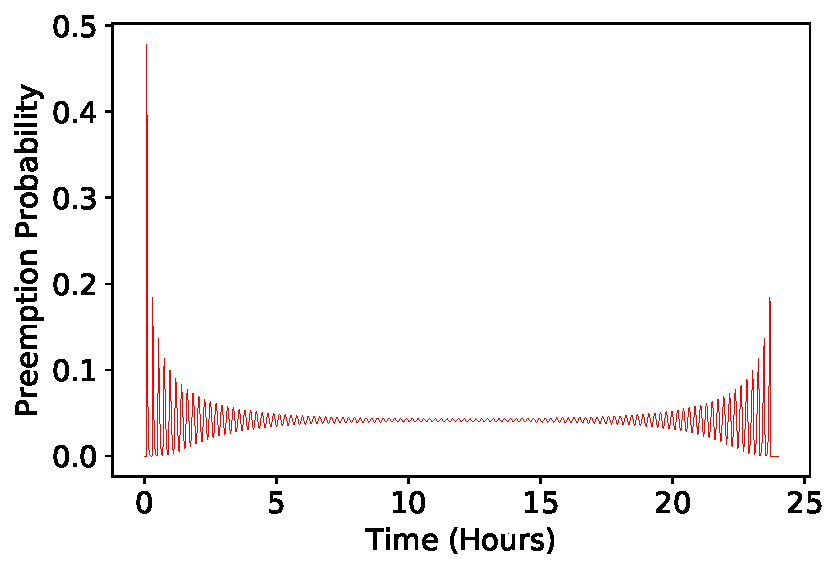
\includegraphics[width=0.3\textwidth]{../graphs/analytical_prob.pdf}
  \caption{Preemption probability computed using the partition function defined for a simple constrained system is also bathtub shaped.}
  \label{fig:partfun}
\end{figure}

 


%%% Local Variables:
%%% mode: latex
%%% TeX-master: "paper"
%%% End:

%%%%%%%%%%%

\begin{comment}
\subsection{Elsewhere: Role of Cloud Providers: Analogy to Constrained Physical Systems}

The bathtub-shaped distribution of the preemption probability is essential to capture the empirical data with higher accuracy compared to other models. We want to probe the following question now: how much of this unique shape is enforced by the cloud provider, and how much is dictated by assuming that (akin to other cloud providers such as EC2), preemptions of Google Preemptible VMs are placed along the timeline of 24 hours with uniform probability? We make the question more precise and inject a relatively harmless assumption: if the cloud provider decides to ``place'' $N$ preemptions within the temporal boundary of interval $L$ with flat probability distribution ($\mathscr{P}(e_1, e_2, \ldots e_N)$ = 1 whenever legal) such that the preemptions are mutually exclusive (that is there is a finite non-zero waiting time between preemptions), what is the probability of finding a preemption at time $t$? Naively, deducing from $\mathscr{P}$, one may expect $p(t)$ to be 1 for $t\in L$, or a constant (flat) distribution. However, intruigingly, this is not true. Thus, as we discuss in more detail below, the cloud provider may have the simplest of preemption policies implemented at their end, and yet give rise to the relatively complex and non-trivial probability to preemption. 

To understand the above assertions with a simple example that sheds further insights into the origins of the bathtub-shaped distribution, we discuss analogous questions in the context of general physical systems of constrained (confined) particles.
These systems are generally analyzed using the theoretical framework of statistical mechanics often complemented with associated particle dynamics simulations. We choose an exactly solvable and simple system of hard (non-overlapping) particles (or beads) confined to move in one dimension within a finite spatial interval to draw interesting connections. 

A simple mapping from the system of temporally-constrained preemptions in the cloud to the system of spatially-constrained particles within one-dimensional confinement can be established by assuming that the cluster management policy requires mutually exclusive preemptions.
This assumption helps cluster management by serializing VM preemptions and making cluster operations easier, and it reduces the challenges associated with reacting to simultaneous preemptions. 
The preemption events become hard particles that cannot overlap. The preemption probability distribution gets mapped to the density of $N$ particles, each modeled as a one-dimensional ``sphere'' of width $\sigma$, confined in a 1-dimensional interval (line segment) of length $L$. $L$ can be considered as corresponding to the deadline interval of 24 hours. $\sigma$ is equivalent to the length of the critical section, which is related to the preemption warning (30 seconds for Google PVMs). 

The particles are placed, one after another, at random positions. Configurations where any overlap is generated are not included. Thus particles will be placed with a flat probability distribution.
The question we are trying to simulate with this set up is the familiar one noted above: what is the probability $P(x)$ of finding a preemption at time $x$?

This problem can be solved by first defining a partition function for the system. And doing some neat math.

Present the solution

This distribution is \emph{not} uniform over the interval, but is higher towards the ends of the interval---analogous to the bath-tub shaped nature of preemptions! 

Discuss more.

We thus draw a few critical observations.
An immediate inclincation may be to attribute the observed non-trivial bathtub-shaped preemption probability function to a uniquely designed and structured operational policy of the cloud provider. However, the above analysis shows that even with the vanilla operational policy of placing preemptions with a uniform probability distribution, the finite excluded temporal volume of preemptions in conjunction with the relatively short deadline (which together imply a high average preemption rate) enforce a bathtub-shape-like distribution for finding a preemption at time $t$. Clearly, this does not provide all the subtle features observed in the preemption data as well as the failure model. But even there, it enables to gauge the extent to which the provider has changed the policy on top of the simplest possible implementation.

The analytical framework suggests that the bath-tub shape of the probability distribution is the key characteristic of constrained preemptions.
Therefore, our approach will remain relevant in the face of future changes in preemption characteristics due to changes in cloud usage and operational policies.

\end{comment}

%These systems underlie a variety of phenomena in chemical and materials engineering applications such as ions confined in nanochannels \cite{jing,solis}. 

%In addition to empirically-informed reliability models for preemptions, we also seek to understand \emph{why} their distribution is bathtub shaped in order to provide a mechanistic understanding of preemptions and enhance the model interpretability and generalizability. 
%Our key insight is that the problem of analyzing constrained preemptions can be ``mapped'' to an equivalent problem in statistical mechanics of a physical system, and we can use the theoretical and analytical framework of statistical mechanics to develop a broader understanding of preemptions. 
%This connection to statistical mechanics is given below. 
%To this end, we propose to ``map'' the problem of constrained preemptions to an equivalent problem of constrained many particle physical systems that can be analyzed employing the general theoretical framework of statistical mechanics.

%A simple mapping can be established by assuming that the cluster management policy requires mutually exclusive preemptions.
%This assumption helps cluster management by serializing VM preemptions and making cluster operations easier, and it reduces the challenges associated with reacting to simultaneous preemptions. The preemption events become hard particles that cannot overlap. The probability distribution of $N$ constrained preemption events gets mapped to the density of $N$ randomly distributed particles confined in a 1-dimensional interval of length $L$ (analogous to 24 hours). 
%The particle size is equivalent to the length of the critical section, which is related to the preemption warning (30 seconds for Google PVMs).
%Finding the distribution of non-overlapping (i.e., hard) particles is a central problem in statistical mechanics [5].
%Interestingly, the distribution of particles in a confined interval can be obtained analytically via the exact closed-form expression of the so-called partition function (a common statistical mechanical quantity useful for obtaining the microscopic understanding of macroscopic phenomena).
%This distribution is \emph{not} uniform over the interval, but is higher towards the ends of the interval---analogous to the bath-tub shaped nature of preemptions! 

%The analytical framework suggests that the bath-tub shape of the probability distribution is the key characteristic of constrained preemptions.
%Therefore, our approach will remain relevant in the face of future changes in preemption characteristics due to changes in cloud usage and operational policies.


% \subsection{EC2 spot instances}

% The earliest form of transient cloud instances.
% In addition to having dynamic availability, also have dynamic pricing.
% ``Classic'' spot instances had price determining the availability, and thus a large amount of work was devoted to bidding and analyzing the prices.

% However a recent change to the spot prices no longer allows these assumptions, rendering it impossible to obtain the \emph{exact} availability information from the prices alone.


% \subsection{Google Preemptible VMs}

% Launched in 2015.
% Flat-rate discount of 80\% compared to on-demand servers.
% Interesting availability SLA: the maximum lifetime is 24 hours, and can be preempted earlier as well.

% In this paper we will look at these preemptible VMs and show how to model their availability.
% Given the inability to use EC2 prices, we believe that our approach is more generalizable and robust.


% There are some distinguishing characteristics of GCP preemptible VMs that makes their failure modeling challenging.
% First is their flat pricing and no other signalling information about their preemption rates (MTBFs) that makes server selection difficult.

% \textbf{Modeling Failure Behavior of Preemptible VMs}
% CDF is ``sigmoid'' shaped.
% $P=R*np.sinh((t-t0)/tau) + C$ with a very low $R=10^{-6}, t_0=12, \tau=0.9, C=0.36$

% Basically, this is a mixture of two distributions, the standard exponential distribution, which we call the stabilization rate and an exponentially increasing reclamation rate.

% Preemptible VMs have three availability phases.

% There are many early deaths, then a period of low failure rates, and then the failure rate is exponential with a positive exponent to enable the cloud provider to reclaim the VMs within the deadline (24 hours in the case of Google's Preemptible VMs).








%%% Local Variables:
%%% mode: latex
%%% TeX-master: "paper"
%%% End:
